\documentclass[11pt]{article}
\usepackage{geometry}
\usepackage{float}
\usepackage{amsmath}
\usepackage{circuitikz}
\usepackage{amssymb}
\usepackage{amsmath}
\usepackage{mathtools}
\usepackage{tikz}
\usepackage{tikz-3dplot}
\usepackage{cite}
\usepackage{url}
\usetikzlibrary{chains}
\usetikzlibrary{decorations.pathmorphing,calc,positioning,arrows.meta}
\usetikzlibrary{positioning,shapes,arrows.meta,calc}
\usepackage{graphicx}
\usepackage{xcolor}
\usepackage{parskip}
\usepackage{braket}

\title{Measurement of the Zeeman Effect via a Fabry-Pérot Interferometer}
\author{Spandan Suthar and Antoni Gonzalez}
\date{February 2, 2026}

\geometry{margin=1in}

\begin{document}

\maketitle

\section{Introduction and Background}

Atoms can be attributed a net spin angular momentum $\vec S$ resulting from their electrons' aggregate intrinsic angular momenta and a net orbital angular momentum $\vec J$ resulting from their electrons' motion around their
parent nucleus. In a weak magnetic field $\vec B$, these two angular momenta couple. The result is a net angular momentum vector $\vec J$ that is quantized instead of either of its $\vec L$ and $\vec S$ consitiuents.

The atom's angular momentum $\vec \mu_J$ is a function of this coupled $\vec J$, resulting in a quantized
set of values. The relative orientation of $\vec \mu_J$ and $\vec B$ produce a quantized set of possible energies around the original zero-field energy level. Assuming a regime of weak magnetic fields (where magnetic potential energy contributions are much smaller than any energy contributions due to spin-orbit coupling), this energy shift is given to first order in $|\vec B| =B$ by the expectation of the Zeeman Hamiltonian term:

\begin{equation}
\braket{\hat {H_Z}} = -\braket{\hat {\boldsymbol \mu} \cdot {\mathbf B} } \approx \mu_B g_J \mathbf B \cdot \braket{\hat {\mathbf J}} = \mu_B g_J B M_J
\label{eq:H_zeeman}
\end{equation}

\begin{equation}
    \mu_B = \frac{e\hbar}{2m_e}
\label{eq:magneton}
\end{equation}

where $\mu_B$ is the Bohr magneton, $g_J$ is the Landé g-factor for the state, $\braket{\hat {\mathbf J}} \equiv \vec J$ is the expectation value of the total angular momentum operator $\hat {\boldsymbol J}$, $M_J$ is the magnetic quantum number corresponding to the projection of $\vec J$ along the direction of $\vec B$, $e$ is the elementary charge, $\hbar$ is the reduced Planck constant, and $m_e$ is the electron mass.

Electrons can transition from one state to another, resulting in the emission or absorption of photons with wavelengths corresponding to the energy difference between the states:

\begin{equation}
\ket{\gamma, L, S, J, M_J} \rightarrow \ket{\gamma, L', S, J', M_J'}
\label{eq:general_transition}
\end{equation}

where $L$ is the atom's total orbital angular momentum quantum number, $S$ is the atom's total spin quantum number, $M_J$ is the atom's total magnetic quantum number, $J$ is the atom's net angular momentum quantum number, and $\gamma$ represents other values necessary to uniquely identify the states. These quantum numbers have values constrained to the following ranges:

\begin{table}[H]
\centering
\label{tab:quantum_number_values}
\begin{tabular}{cll}
\hline
\textbf{Quantum number} & \textbf{Symbol} & \textbf{Range} \\
\hline
Spin & $S$ 
& $\set{0, \tfrac12, 1, \tfrac32, \dots}$ \\

Orbital angular momentum 
& $L$ 
& $\set{0,1,2,\dots}$ \\

Total angular momentum 
& $J$ 
& $\set{|L-S|,\dots,L+S}$ \\

Magnetic quantum number 
& $M_J$ 
& $\set{-J,\,-J+1,\dots,J}$ \\

\hline
\end{tabular}
\end{table}

For the purposes of this experiment, the state's electron configuration is a sufficient stand-in for $\gamma$. 

Emissions and absorptions of electrons are modeled through a Hamiltonian term characterizing interactions with an electromagnetic field, whose symmetries impose selection rules on the allowed transitions:

\begin{table}[H]
\centering
\label{tab:E1_selection_rules_ops}
\begin{tabular}{cll}
\hline
\textbf{} & \textbf{Operator} & \textbf{Selection rule} \\
\hline
1 & $\hat{\mathbf{S}}^2$ 
  & $\Delta S = 0$ \\

2 & $\hat{\mathbf{L}}^2$ 
  & $\Delta L = \pm 1$ \\

3 & $\hat{\mathbf{J}}^2$ 
  & $\Delta J = 0, \pm 1$ \quad ($J=0 \nleftrightarrow J'=0$) \\

4 & $\hat{J}_z$ 
  & $\Delta M_J = 0, \pm 1$ \\

5 & $\hat{\Pi}$ (parity) 
  & $\Pi' = -\Pi \;\;(\Delta \Pi \neq 0)$ \\

\hline
\end{tabular}
\end{table}


In the subset of transitions where the initial and final states of the electron have zero net intrinsic angular momentum $\vec S = 0$, $\vec J$ reduces to $\vec L$:

\begin{equation}
\ket{\gamma, L, S=0, J=L, M_J} \rightarrow \ket{\gamma', L', S=0, J'=L', M_J'}
\label{eq:normal_transition}
\end{equation}

In the weak-field regime, the degeneracy splitting of atomic energy levels due to an external magnetic field is known as the Zeeman effect. For atoms whose initial and final states satisfy $\vec S = 0$, this splitting is known as the normal Zeeman effect---while cases in which $\vec S \neq 0$ are known as the anomalous Zeeman effect. A family of transitions that exhibits the normal Zeeman effect is the $5s5d \rightarrow 5s5p$ transition in neutral cadmium (Cd I):

\begin{equation}
\ket{\gamma=5s5d;\,L=2,\,S=0,\,J=2,\,M_J}
\;\longrightarrow\;
\ket{\gamma'=5s5p;\,L'=1,\,S'=0,\,J'=1,\,M_J'}
\label{eq:cd_transition}
\end{equation}

In spectroscopic notation, this transition family is denoted $5s5d\;{}^{1}D_{2} \;\longrightarrow\;5s5p\;{}^{1}P_{1}$. Following \ref{tab:quantum_number_values}, the former state splits into 5 substates with $M_J \in \set{ -2, -1, 0, 1, 2}$, while the latter splits into 3 substates with $M_J' \in {-1, 0, 1}$.

The degeneracy splitting of the $5s5d\;{}^{1}D_{2}$ and $5s5p\;{}^{1}P_{1}$ allows for three disctint changes in energy where there used to be one, resulting in three possible wave lengths of emitted photons. Because the energy shift $\braket{\hat {\mathbf H}_Z}$ is proportional to $M_J$ (Eq. \ref{eq:H_zeeman}), the possible changes in energy are proportional to $\Delta M_J$ over the transition. The selection rules of Table \ref{tab:E1_selection_rules_ops} restrict the allowed values of $\Delta M_J$ to $\set{-1, 0, 1}$, resulting in three possible energy changes (and thus three possible emitted photon wavelengths) for the $5s5d\;{}^{1}D_{2} \;\longrightarrow\;5s5p\;{}^{1}P_{1}$ transition, illustrated in Figure \ref{fig:energy_levels}.

% Include the TikZ diagram from the external file
\begin{figure}[H]
    \centering
    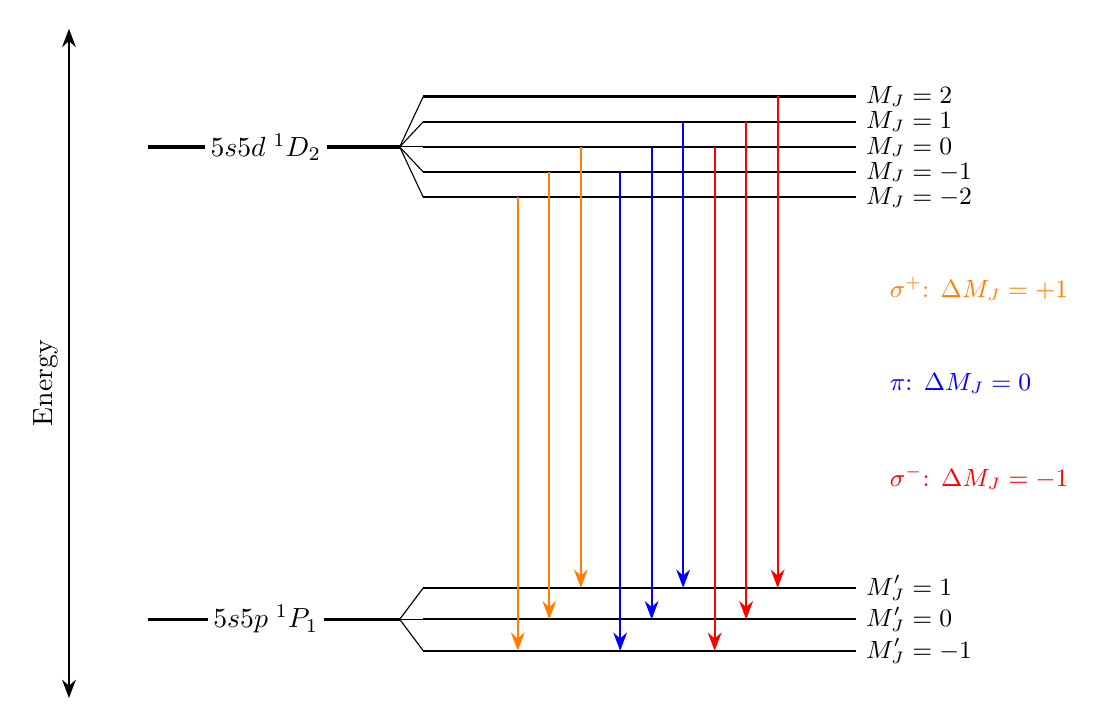
\begin{tikzpicture}[>=Stealth]

% Define vertical positions
\def\upperenergy{6}
\def\lowerenergy{0}
\def\splitupper{0.8}
\def\splitlower{0.6}

% Define horizontal positions
\def\leftstart{0}
\def\middlesplit{3.5}
\def\rightend{9}

% Upper state (5s5d, J=2)
\draw[very thick, black] (\leftstart, \upperenergy) -- (\middlesplit-0.3, \upperenergy);
\node[fill=white, inner sep=2pt] at (1.5, \upperenergy) {$5s5d\;^1D_2$};

% Upper state splits into M_J levels
\foreach \mj/\offset in {-2/-2, -1/-1, 0/0, 1/1, 2/2} {
    \pgfmathsetmacro\ypos{\upperenergy + \offset*\splitupper/2.5}
    \draw[thick, black] (\middlesplit, \ypos) -- (\rightend, \ypos);
    \node[right, font=\small] at (\rightend, \ypos) {$M_J = \mj$};
}

% Draw branching from unsplit to split (upper)
\draw[black] (\middlesplit-0.3, \upperenergy) -- (\middlesplit, \upperenergy + 2*\splitupper/2.5);
\draw[black] (\middlesplit-0.3, \upperenergy) -- (\middlesplit, \upperenergy + 1*\splitupper/2.5);
\draw[black] (\middlesplit-0.3, \upperenergy) -- (\middlesplit, \upperenergy);
\draw[black] (\middlesplit-0.3, \upperenergy) -- (\middlesplit, \upperenergy - 1*\splitupper/2.5);
\draw[black] (\middlesplit-0.3, \upperenergy) -- (\middlesplit, \upperenergy - 2*\splitupper/2.5);

% Lower state (5s5p, J=1)
\draw[very thick, black] (\leftstart, \lowerenergy) -- (\middlesplit-0.3, \lowerenergy);
\node[fill=white, inner sep=2pt] at (1.5, \lowerenergy) {$5s5p\;^1P_1$};

% Lower state splits into M_J' levels
\foreach \mj/\offset in {-1/-1, 0/0, 1/1} {
    \pgfmathsetmacro\ypos{\lowerenergy + \offset*\splitlower/1.5}
    \draw[thick, black] (\middlesplit, \ypos) -- (\rightend, \ypos);
    \node[right, font=\small] at (\rightend, \ypos) {$M_J' = \mj$};
}

% Draw branching from unsplit to split (lower)
\draw[black] (\middlesplit-0.3, \lowerenergy) -- (\middlesplit, \lowerenergy + 1*\splitlower/1.5);
\draw[black] (\middlesplit-0.3, \lowerenergy) -- (\middlesplit, \lowerenergy);
\draw[black] (\middlesplit-0.3, \lowerenergy) -- (\middlesplit, \lowerenergy - 1*\splitlower/1.5);

% Transition arrows - three distinct regions with symmetric margins
% Branch region spans from 3.5 to 9.0 (width = 5.5)
% Arrow region spans from 4.7 to 8.0 (width = 3.3, margins = 1.2 on each side)
% Ordered left-to-right corresponds to bottom-to-top

% LEFT REGION: Orange $\sigma^+$ transitions ($\Delta M_J = +1$)
% M_J = -2 → M_J' = -1
\draw[->, thick, orange] (4.7, \upperenergy - 2*\splitupper/2.5) -- (4.7, \lowerenergy - 1*\splitlower/1.5);
% M_J = -1 → M_J' = 0
\draw[->, thick, orange] (5.1, \upperenergy - 1*\splitupper/2.5) -- (5.1, \lowerenergy);
% M_J = 0 → M_J' = 1
\draw[->, thick, orange] (5.5, \upperenergy) -- (5.5, \lowerenergy + 1*\splitlower/1.5);

% MIDDLE REGION: Blue $\pi$ transitions ($\Delta M_J = 0$)
% M_J = -1 → M_J' = -1
\draw[->, thick, blue] (6.0, \upperenergy - 1*\splitupper/2.5) -- (6.0, \lowerenergy - 1*\splitlower/1.5);
% M_J = 0 → M_J' = 0
\draw[->, thick, blue] (6.4, \upperenergy) -- (6.4, \lowerenergy);
% M_J = 1 → M_J' = 1
\draw[->, thick, blue] (6.8, \upperenergy + 1*\splitupper/2.5) -- (6.8, \lowerenergy + 1*\splitlower/1.5);

% RIGHT REGION: Red $\sigma^-$ transitions ($\Delta M_J = -1$)
% M_J = 0 → M_J' = -1
\draw[->, thick, red] (7.2, \upperenergy) -- (7.2, \lowerenergy - 1*\splitlower/1.5);
% M_J = 1 → M_J' = 0
\draw[->, thick, red] (7.6, \upperenergy + 1*\splitupper/2.5) -- (7.6, \lowerenergy);
% M_J = 2 → M_J' = 1
\draw[->, thick, red] (8.0, \upperenergy + 2*\splitupper/2.5) -- (8.0, \lowerenergy + 1*\splitlower/1.5);

% Energy axis
\draw[<->, thick] (-1, \lowerenergy - 1) -- (-1, \upperenergy + 1.5);
\pgfmathsetmacro\midheight{(\upperenergy + \lowerenergy)/2}
\node[rotate=90, fill=white, inner sep=2pt] at (-1.3, \midheight) {Energy};

% Transition labels
\pgfmathsetmacro\midtrans{(\upperenergy + \lowerenergy)/2}
\node[orange, font=\small, right] at (9.3, \midtrans + 1.2) {$\sigma^+$: $\Delta M_J = +1$};
\node[blue, font=\small, right] at (9.3, \midtrans) {$\pi$: $\Delta M_J = 0$};
\node[red, font=\small, right] at (9.3, \midtrans - 1.2) {$\sigma^-$: $\Delta M_J = -1$};

\end{tikzpicture}
    \label{fig:energy_levels}
    \caption{}
\end{figure}

The transitions are grouped by their energy differences $\Delta E$---equivalently, their $\Delta M_J$ values--- and thus correspond to three distinct spectral lines. Cadmium atoms can therefore undergo, in order of increasing energy difference, $\sigma^-$, $\pi$, and $\sigma^+$ transitions. These correspond to $\Delta M_J = -1$, $0$, and $1$, respectively, and yield photons with short, moderate, and long wavelengths.


Note that because a photon is massless, it can never have a frame in which it is at rest; a photon has a momentum in all relativistic frames. Thus, the only generators of \textit{pure} rotations---i.e., operators corresponding to the photon spin---must produce rotations about the photon's momentum $\vec p$ to prevent changing the direction of the photon's momentum. This confines them to $\text{SO(2)}$. In conjunction with a photon's status as a spin-1 boson, this implies that the only allowed eigenvalues of the photon's spin operator $\hat{h}$ are $\pm \hbar$. Taken with the fact that a $\pi$-transition emits a photon with state $\ket \pi = \frac{1}{\sqrt{2}} \left ( \ket {\sigma^+} + \ket {\sigma^-} \right )$ with a spin of 0 in expectation, this means that the emission of appropriate photons can exactly satisfy a conservation of angular momentum constraint applied to the atom-photon system during a transition.

\begin{equation}
    \bra{\sigma^\pm} \hat{h} \ket{\sigma^{\pm}} = \pm \hbar
    \quad 
    \bra{\pi} \hat{h} \ket{\pi} = 0
\end{equation}

% Spin must be intrinsic physical and thus Lorentz invariant
% Spin components can mix for particles that have rest frames (massive particles) but total spin should be agreed-upon; the total spin is intrinsic but basis changes can cause component mixing (observer-to-observer disagreement)
% The only axis along which a measured spin can be Lorentz invariant is along the direction of motion--because photon cannot be at rest
% 

% The only operator that cannot change the eigenvalue of the photon's generator of translation must be the rotation operator about the axis of motion (corr. helicity)
% Thus those angular momentum eigenvalues must be defined along the axis of motion strictly


% SO(3) is a subgroup of the Lorentz group

\section{Goal}
\section{Procedure}
\section{Results and Analysis}
\section{Discussion}
\section{Conclusion}

\end{document}
